\documentclass{article}

\usepackage{graphicx} % Required for the inclusion of images

\setlength\parindent{0pt} % Removes all indentation from paragraphs
\usepackage[utf8x]{inputenc}

\usepackage{times} % Uncomment to use the Times New Roman font
\usepackage{siunitx}
\usepackage{textgreek}



\title{Amplificazione RealTime PCR. Estrazione proteine totali \\ (Esercitazione n° 10)} % Title

\author{Litterini S. \\Giulio B. \\Cracco A.\\Buzzolan T. } % Author name

\date{20 Aprile 2018} % Date for the report

\begin{document}

\maketitle


\section{Sommario}

\subsection{Scopo}


Questa esperienza ha come scopo quello di amplificare un cDNA tramite la PCR real time. Inoltre vediamo l'estrazione delle proteine e la loro quantificazione al Qubit 3.


\subsection{Cenni teorici}

La PCR real time è una particolare PCR che ci permette di amplificare e
contemporaneamente quantificare il DNA in tempo reale osservando la fluorescenza ad ogni iterazione.
Pargonando due campioni diversi e' possibile stabilire il rapporto tra le quantita' iniziali della sostanza.
Per rendere il campione fluorescente si utilizza una sonda composta da una colorante
fluorescente (Responser) e da un Quencer che assorbe l'energia della fluorescenza.
La sonda si lega tra i due primer del gene.
Quando la sonda viene degradata (dall'attivita' esonucleasica della TAQ-polimerasi)
il Quencer e il Responser si separano, in questo modo il Responser e' libero di emettere
la fluorescenza che e' quindi misurabile.

\section{Strumenti e materiali utilizzati}

\begin{itemize}
\item Guanti in lattice
\item 2xProvette Eppendorf (1.5mL)
\item Assay tube (500ul)
\item Micropipette (100-1000  e 2-200 microlitri  )
\item Qubit 3 (per quantificare le proteine)
\end{itemize}


\section{Soluzioni utilizzate}
\begin{itemize}
\item cDNA
\item Pellet cellulare per l'estrazione delle proteine
\item RIPA buffer
\item Working solution
\item
\end{itemize}



\begin{itemize}

\item miniprep del pUC18
\item cellule competenti
\item LB liquido

\end{itemize}



\section{Procedimento}

\subsection{Amplificazione RealTime PCR}
\begin{itemize}
\item Prendere il cDNA dall'esperienza precedente
\item Utilizziamo questa quantita' di reagenti per un volume finale di 40 ul diviso in due pozzetti da 20ul: \\
\begin{tabular}{c c c c}
\hline
Reagente & Concentrazione & $\mu$l/pozzetto & ul 2 pozzetti \\
\hline
MasterMix & 2X & 10ul & 20ul \\
Sonda TaqMal & 20X & 1ul & 2ul \\
H$_2$O & 1X & 7ul & 14ul \\
cDNA & 1X & 2ul & 4ul \\
\end{tabular}
\item Aliquotare ogni reagente in un'Eppendorf da 1,5ml.
\item Spostare ogni reazione nei pozzetti (appoggiarsi al bordo per essere pi\'u precisi)
\item Sigillare con l'adesivo ottico
\item Centrifugare brevemente
\item Avviare la reazione di amplificazione \\
Questi sono i parametri del termociclatore:\\
\begin{tabular}{c c c c c}
\hline
Parametro & Incubazione UNG & Attivazione polimerasi &
\multicolumn{2}{c}{PCR (40 cicli)} \\
% Hold Hold Denaturazione Allealing/estensione
Temperatura & 50C & 95C & 95C & 60C \\
Tempo (mm:ss) & 02:00 & 10:00 & 00:15 & 01:00 \\
\end{tabular}
\item Attendere il completamento ed analizzare i dati raccolti
\end{itemize}

\subsection{Estrazione delle proteine}
\begin{itemize}
\item Risospendere il pellet cellulare in 100ul di RIPA Buffer addizionato
di inibitori di proteasi con la diluizione: \\
\begin{tabular}{c c c}
Reagente & Concentrazione & Quantit\'a \\
RIPA buffer & 1X & 96ul \\
Inibitori & 25X & 4ul \\
& & TOT = 100ul
\end{tabular}
Il buffer di lisi serve a rompere le cellule

\item Incubare per 45' in ghiaccio
\item Centrifugare per 40'' a 4C
\item Prelevare il surnatante (contenente le proteine) in una nuova eppendorf
\item Conservare in ghiaccio
\end{itemize}

\subsection{Quantificazione proteine con Qubit 3}
\begin{itemize}
\item Preparare la Working Solution, che servir\'a sia per la taratura dello strumento
che per la misurazione della quantit\'a di proteine. Nel nostro caso lo strumento era
gi\'a stato tarato, quindi dalla tabella escludiamo le 3 dosi per la taratura.

\begin{tabular}{c c c}
Reagente & Quantit\'a 1 dose & Quantit\'a 10 dosi \\
Qubit protein reagent & 1ul & 10ul \\
Qubit protein buffer & 199ul & 1990ul \\
 & TOT = 200ul & TOT = 200ul \\
\end{tabular}

\item Aliquotare 190ul di Working Solution in un AsseyTube da 500ul
\item Aggiungere 10ul di proteine, invertire il tubo 10 volte e centrifugare brevemente
\item Lasiare la miscela al buio per 15'
\item Leggere l'emissione del fluoroforo

\end{itemize}

\begin{figure}
  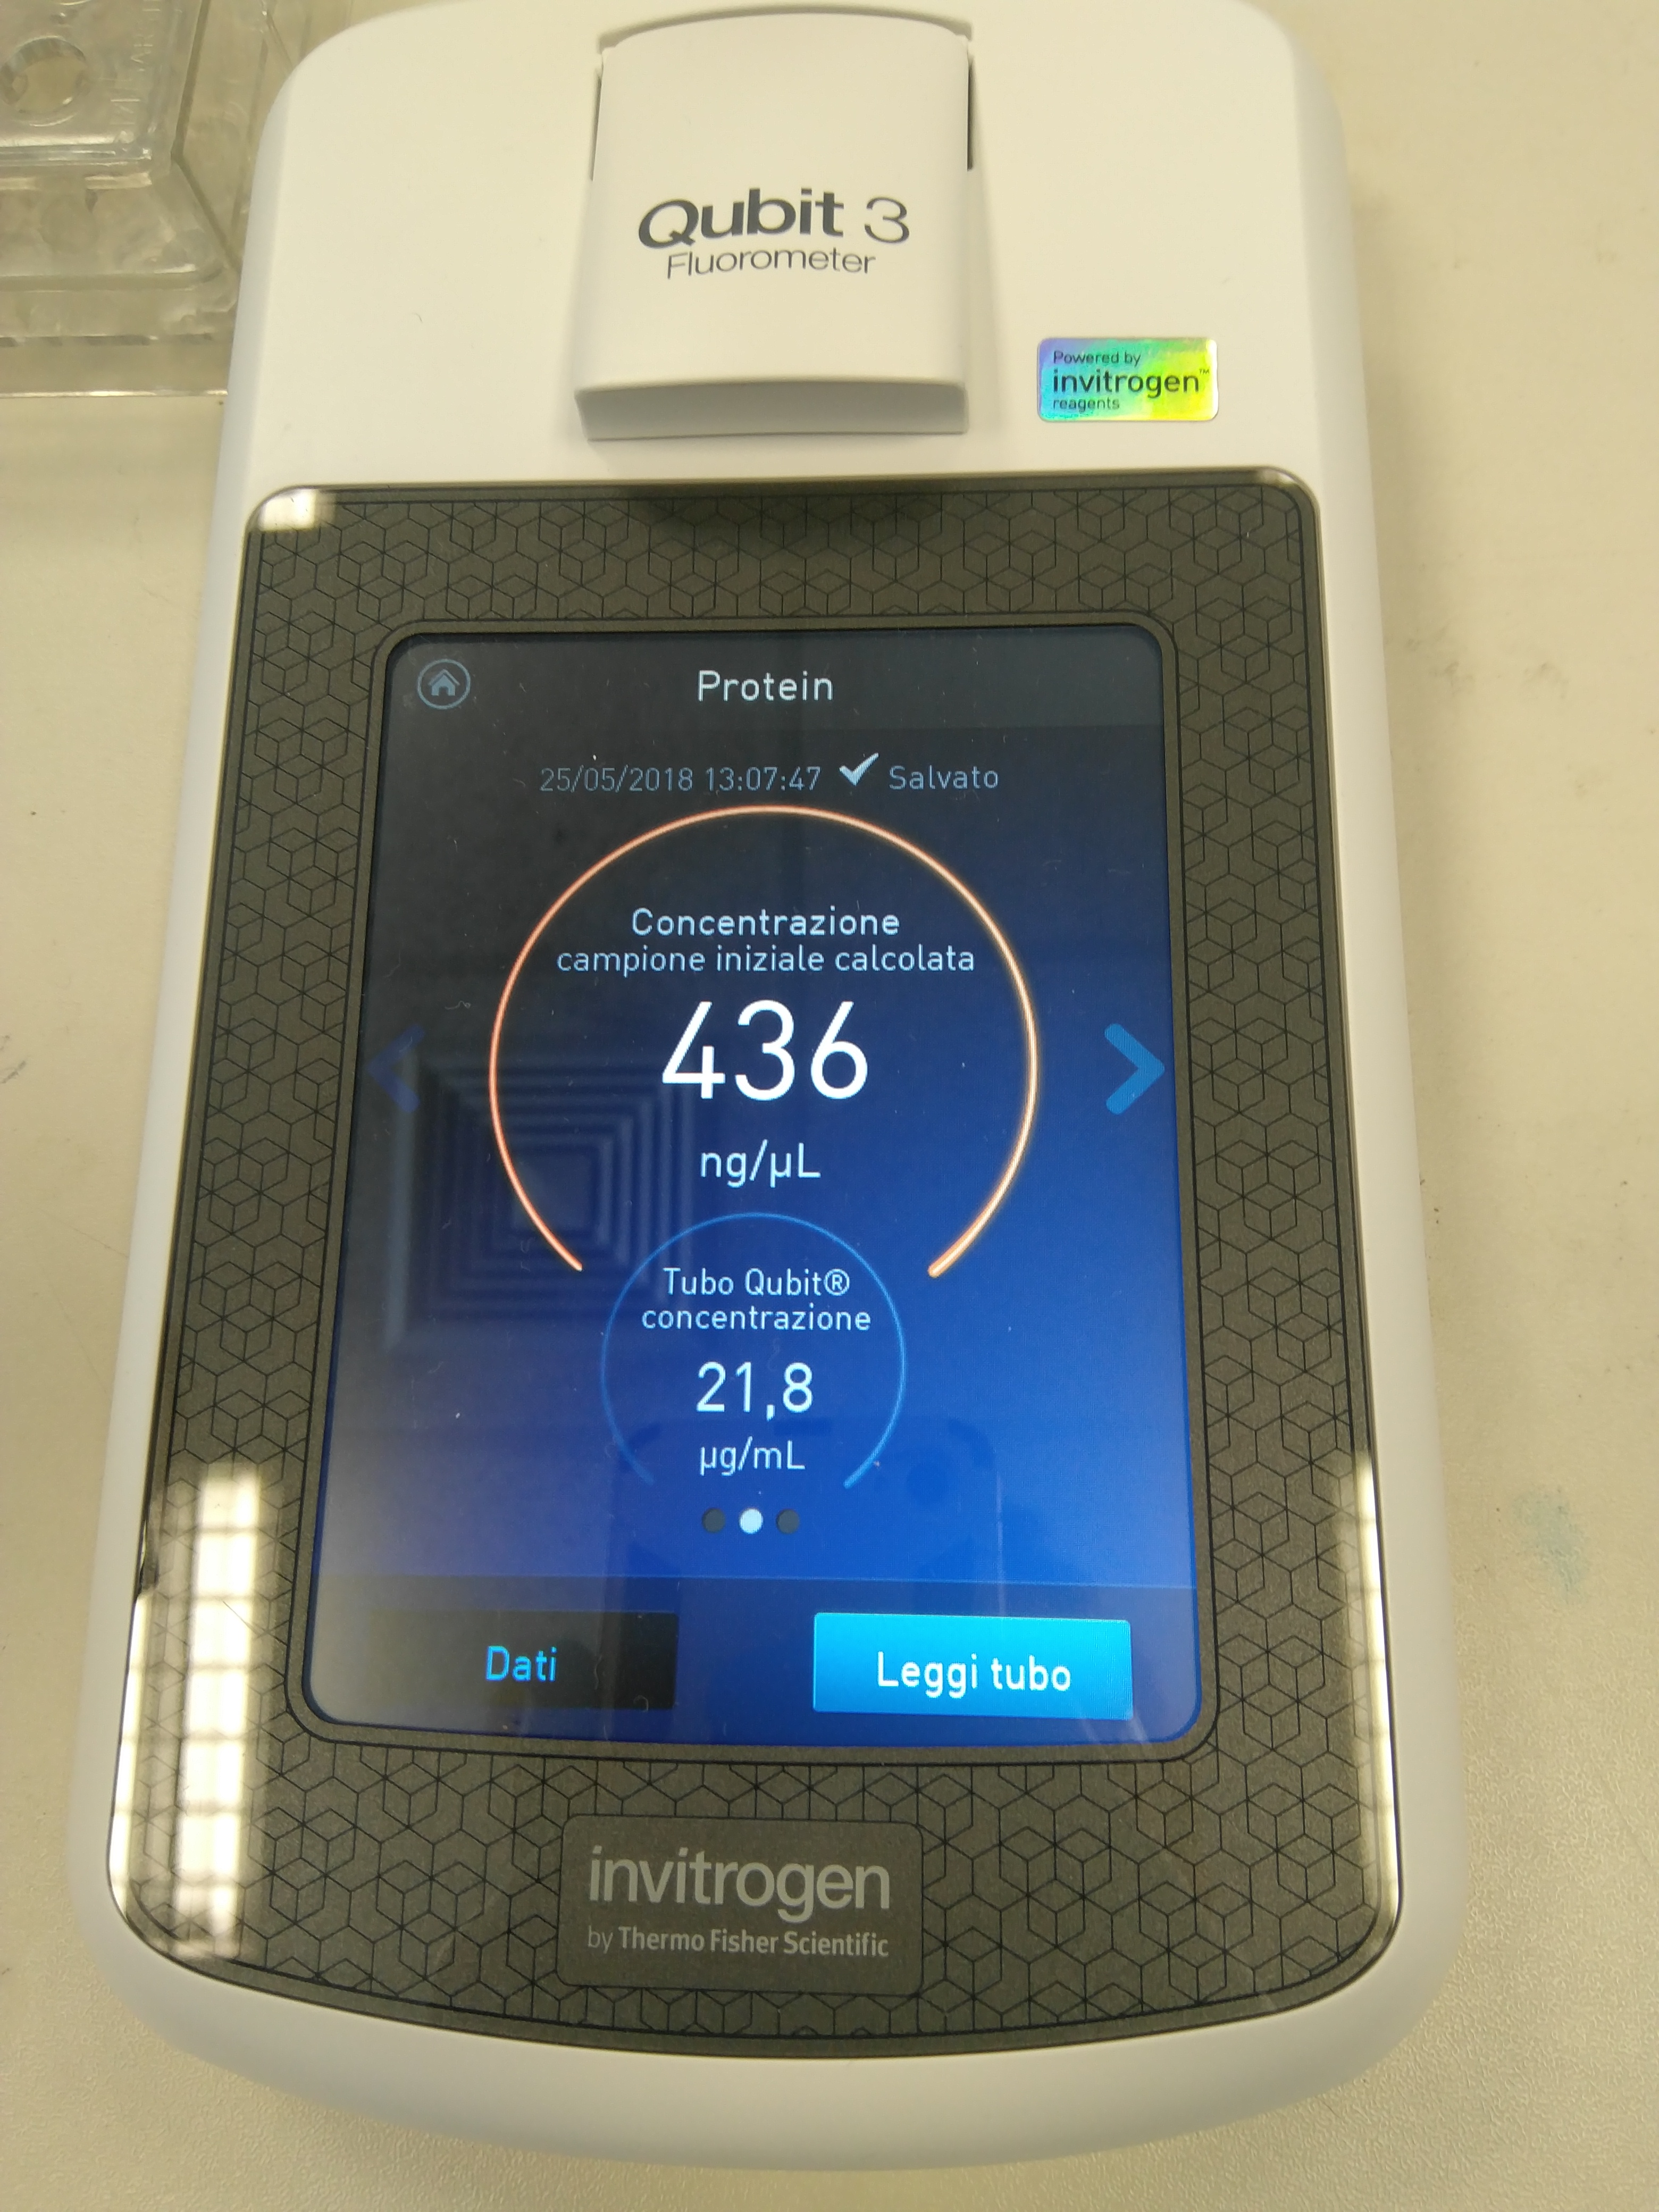
\includegraphics[width=\linewidth]{qubit3.jpg}
  \caption{Risultati della quantificazione delle proteine.}
  \label{fig:qubit3}
\end{figure}

\section{Risultati e Conclusioni}
RealTime PCR:
Come risultato abbiamo osservato un grafico con una curva di amplificazione con le quantit\'a ad ogni ciclo.
Abbiamo visto che ha un andamento logaritmico
Tracciando una linea orizzontale e' possibile verificare la soglia di fluorescenza.\\

Quantificazione Proteine:
La concentrazione ottenuta per le nostre proteine e' di 436 ng/ul. Visto che eravamo partiti con una
quantita' di 100ul, e 10ul sono stati utilizzati per la quantificazione, moltiplicando per 90ul possiamo
ottenere la quantita' totale di proteine del nostro campione.

\end{document}
